ABSTRACT

%****************************************
% SAMPLE ABSTRACTS

% Bu çalışmada, ne kadar itici bir kavram olsa da, çöplük olgusunun çirkinlikten güzelliğe ulaşarak estetik bir haz uyandırması amaç edinilmiştir. Iticici gözüken bir konunun resim diliyle anlatımı ile tersine çekici ilginç bir sanat konusu olabileceğinin somutlaştırılması amaçlanmıştır. Sanatçı bir anlamda doğada yaşamda bulunan küçük ayrıntıları, sanatsal bir gözle yaklaşarak gösterebilendir. Resim için konu denince hep bildik tanıdık nesneler, belli bir düzenleme anlayışı (Natürmort) ya da idealize edilmiş konular, temalar akla gelir. Oysa önemsiz gibi gözüken itici karmaşık konular bile sanatsal kaygılarla ele ahnabilmelidir. Önemli olan, bu konalara estetik yaklaşım ve izlenen anlatım yol ve teknikleridir. Özgün baskı dallarından kazı resim (gravür) tekniğinin ele alınan konunun görselleştirilmesinde, anlatımında en uygun teknik olmasıdır. Çünkü her sanatçı kendi doğasına en uygun olan teknik ve malzemelerin olanaklarıyla kendini en rahat biçimde ifade etme olanağı bulur. Kendine özgü bir biçim ve anlatım diliyle dile getirmek gerçekleştirmek çabalan özgünlüğü yakalamak içindir. Bu çalışmada özgünlüğü yakalamak, çöplük olgusunun oluşturduğu dinamik yapı, objelerin biçimlerine bağlı kalmadan plastik dille görselleştirilmiştir. Seçilen teknik doğası gereği raslantısal tadlarada olanak vermektedir. Oluşturulan resimlerde durağan bir dengeden çok dinamik biçim ilişkilerine dayanan gerilimli bir etkinin yakalanması amaçlanmıştır.

% ON THE RELATIONSHIP BETWEEN IMAGES AND WORDS AND THEIR RELATION TO BODY AND PERCEPTION
% Prehistoric man created a mark and throughout the history this mark evolved and bifurcated into two: a word and an image. While images were cherished, words were set apart from images. 
% This thesis attempts to look at the relationship between images and words through seeking their connection to perception and body. It investigates how image-word dichotomy occurred and how this dichotomy obscured the connection between writing and body. The thesis also examines different approaches to overcome this phenomenon in the context of Modern Art. 
% By examining my artwork within this framework, it argues that it is possible to embody the inseparable relationship between images and words through reconnecting with the body’s primordial existence.

% ALTERNATIVE PHOTOGRAPHY IN THE DIGITAL AGE: PERFECT PHOTOGRAPHS IN AN IMPERFECT WAY
% This thesis explores the possibility of an alternative future of photography from the union of digital and chemical domains of the photographic medium. The historical photographic processes known as Cyanotype, Salt print and Vandyke Brown are employed for this project in conjunction with the modern inkjet printer produced digital negatives. 
% As being highly sensitive to the variables during the process, each alternative photographic print exhibits a visual uniqueness. In this aspect, there is conceptual correlation with the visual uniqueness of alternative photographic processes and the visual uniqueness of albinism. Emphasizing the human element in subject, vision and craft of making photographs, this project aims to produce unique photographs of a visually unique subject.

% LAND ART ON THE BORDER BETWEEN TOPOLOGY AND ATOPOLOGY
% The purpose of this study is to discuss the Land Art movement from a topological and atopological perspective. In order to establish an extensive understanding of the matters of topology and atopology, Arkady Plotnitsky’s formalization of quasi- mathematical thinking, which is derived from Jacques Derrida’s philosophy, is treated in detail. The artistic stance, Robert Smithson, as a major figure of Land Art movement is analyzed both from the artistic and the theoretical perspectives. Thereafter, an algebraic reading of the Smithsonian conceptualization is executed in order to illuminate the liaison between the Land Art movement and the matters of topology and atopology. Finally, the thesis project, Nonlocalizable Displaced Mirrors depicts the whole attitude, which is taken throughout the study, towards the issue of Land Art on the Border between Topology and Atopology.

%........................................


INTRODUCTION

% Bence introductionda çöpün farklı şekillerde ele alınabileceğini bir şekilde göstermek gerekli. Burdaki genel geçer yaklaşımdan bahsetmek gerekli.
% Ele aldığımız çöp insanların çöpleri, günlük kullanımdaki çöpler. Çok da değerli olmayan yerine yenisi koyabileceğimiz çöpler. 

% Western societies from periods where manual labor and long struggle required in production process and materials are reused and transformed again and again, have reached to periods where production process speeds up and becomes more accessible. Consumption habits have changed radically and have created piles of trash that is not obvious how to reuse them. In this work the practice and process of reusing and transforming trash which is an alternative to today's existing production and consumption habits is investigated. Stages and expression of this practice is examined with my artwork in the context of art.

% Konunun dikkat çekici ilginç kısımları. Interesting points of the topic. Facts about the trash. Changes through the time.
% Konu hakkındaki temel bilgiler.
% Konunun ele alınan kısmı.

% Çöp ve dönüşümden bahsetmek gerekli. Çöp nedir? Dönüşüm nedir? Çöpün bir dönüşümü var mıdır? Var ise bu nasıl bir şeydir? 
% Introduce as an discussion. Trash is valueless? really? is it just a sculpture? Tons of different approaches to the trash. 

% Bu trash in every sıralamasını neden yapıyorum? Genel bir çerçeve çizmekten çok aslında evrensel bir konu olduğuna değinmiş oluyorum. Peki bu çok açık bir şey mi? Yani aslında çok da açık olmayan bilgilerek vererek yaparsam olmayabilir. Evrensel olmasının benim için ne önemi var. Yaşamımızın bir parçası demek. Tamam da buna karşı bir şey mi var. Ben göremiyorum açıkcası. Herkes bunu biliyor. Farkında mıyız. Ama farkında olmak istemediğimiz bir şey ki sürekli kendimizden uzaklaştırıyoruz. O zaman bu gerçekleri aslında ne kadar biliyoruz. Ama bunları bilmek böyle davranmamız gerektiği anlamına mı gelmektedir? Aslında yabancı olmadığımız ama uzak durduğumuz bir konu. Belki de sırf bu yüzden kaçırdığımız bir sürü şey olabilir.

% Aga çöpe farklı yaklaşımlar var. O yüzden background information olarak burada verilebilir ve scope belirlenebilir. Tam da bu noktada ise purpose kısmına geçilebilir. Çöpe nasıl yaklaşıyorlar falan filan. İşte ben tam da bu noktada sanatta nasıl yaklaşılmıştır dicem. Hatta basitçe sanatta bu tür işlere 


%****************************************
% It is a justification of the work. 
% What is trash? Who does call it trash? 
% Is it possible to transform it? How? Which methods?
%........................................


% Çöpün sanat işlerinde kullanılmasının önemi ne? Bunun karşısındaki şey nedir? Diğer alanlardaki yaklaşımlar bir şey üretemiyor mu? Bu tezin önemi ne? Birilerinin bıraktığı boşluğu doldurmak mı? Ya da benim yaptığım işin önemi ne? 


% ben bunu konuyu bir eylem olarak mı ele alıyorum.


% Önceki işlere değinmek gerekli. Bu alanla ilgili yapılmış. Mesela ne var. İki tane tez buldum aslında tam da bu konuyla ilgili. Önceki işler olacak, yetersiz eksik yanları olacak ve ben onlara belli başlı eklemeler yapacağım.


%****************************************
% Some comments
% Burada önemli olan şey soru veya sorgulanan şey. Bu soru projeye yön verecek. Yazılı tez ise bunun doğrulamasını, üretilen işin kavramsal ve kuramsal çerçevesini belirleyecek. Tartışmalar ne üzerine olmalı bu durumda? 
% The project aims to what? and what needs to justify what it questions? 
% At this point, the question of what will be in the future of photography has to be asked. Bu çok önemli, bir şeyler hazırlayıp neyin sorgulanması gerektiğini sormak gerekli.

% Tipografi ve ideoloji arasında bir ilişki vardır. Fotoğrafın geleceği? Kelime ve imaj arasındaki ilişki, beden ve algı üzerinden incelenebilir? kelime ve imaj arasında bir problem olduğundan bahsediyor. Sanat işlerinde çöp kullanmak toplum tarafından atılan şeyi tekrar kullanılabileceğini gösterebilir. Toplum ve çöp nispeten bir problemli bir durum. Burada bir dert var. Atılan tüketilen manalar var. Sanat bunları provoke mi ediyor. Peki ya ben ne öneriyorum, yani aslında bir şey önermem mi gerekiyor? Sanat ve çöp arasında nasıl bir ilişki vardır? Çöp ile diğer nesneler arasında nasıl bir ilişki vardır? 

% Zaten hali hazırda sanatçılar bunu yapıyorlar, tez aslında bunları inceliyor olabilir ama tez aslında benim işimi inceliyor. İş neyi soruyor ise aslında tez de onu soruyor. Yapılan işlerle sorulan sorular arasında bir bağlantı var. Bu noktada aslında benim işin neyi sorguladığını bulmam gerekli. Çöp dönüştürülebilir, sanatsal bağlamda. (Çok geniş değil mi abi sanatsal bağlamda demek? Çöp de çok geniş bir konu.) Konuyu bir şeklide daraltmak gerekli. Çöp sanat işlerine girmiştir. Çöp dönüştürmek aslında bir artistic acte dönüşüyor. Tezde bunu anlatıyor. Aga bu artisctic act dediğin şey de ne oluyor. Çöp dönüştürmek ne oluyor?

% Çöpe yeni bir alternatif yaşam üretmek gerekli! Neden böyle düşünüyorsun? Çünkü sürekli çöp üretiyorsun ama bir yandan da bundan dert yanıyorsun. Zizek işte bu konuya el basıyor. 

% Aslında hepimiz bir şeyleri dönüştürüyoruz! Neden böyle düşüyorsun? Örnekleri nelerdir? Bricologe bu iddayı destekler mi? Nesnleri üretim amaçlarından farklı amaçlar için kullanmak yeni bir şey değil. (Ama zaten ben sanat amacıyla kullanılmasından bahsedeceğim.) Belki bunu belirtmek için mantıklı olabilir. Ama burada bir farklılık var olamalı. Diğerinden ayıran diyeceğim ama öyle bir fark aramamak gerekli bence. Sanat o farkı yıkmak için uğraşıp duruyor. Belki de bu uğraşa katkısı bu olabilir bu işin. Bir şeyleri dönüştürme potansiyellerimiz olduğunu düşünebiliriz. Dönüştürme dediğimiz şey aslında hangi noktada açığa çıkıyor. Bir ihtiyaç anında, kaçış anında, ya da yeni alternatifler ararken mi?

% Çöpün dönüştürülmesi ne olaki? Buna bir şekilde girişte yer vermek gerekli. Çöpün market içindeki hareketi mi? Ya da aslında çöpün yaşamı. Belki de bu olabilir. Çöpün nasıl oluştuğu vs. Fabrikada üretilmesi. İnsanlara dağıtılması. Ve sonra çöp olması. Çöp dağları oluşması. Çöp kutusunda yer alması. Neler yok ki çöp kutusunda. Bir sanatçı çöp kovasına attığı sanat işleri. Sanat işleri çöplükleri vs. Çöp kavramı aslında o kadar çok şey için geçerli ki? İşte bu çok çeşitli çöp kavramını ele almak gerekli. Yani objeler bir şekilde farklı konumlarda mekanlarda yer değiştiriyorlar. Bazen çöp oluyorlar bazen değerli vs.

% Bir bir çeşit çöp var. Bunlar binbir çeşit davranış sonucunda oluşuyorlar. Bir işlemin sonunda ortaya çıkan son ürün. Çöp konumuna gelmesi vs. Kime göre çöp neye göre çöp. Ama işte ortada bir konsensus yok. Başkaları da farklı şekilde görüyor. Birine göre çöp diğerine göre ise bir hazine.

% Dönüşmek ne oluyor peki bu durumda. Bir durumdan başka bir duruma geçmesi. Farklı bir anlam, amaç kazanması olabilir mi? Mesela pisuvar dönüşmüş müydü? Gazeteyi kolajda kullandığım zaman gazeteyi dönüştürmüş mü oluyorum? Hangisi dönüştü? Zaten buradaki açık bir şekilde açığa çıkıyor aslında. Her ikisi de dönüşmüş oluyor. Farklı bir kullanım alanı bulmak. Farklı niyetlerle kullanmak olabilir belki de. Bir şeyin ne zaman dönüştüğünü iddia edebilirsin.

% Agnes varda neyi anlatıyor: Toplayıcılık hala devam ediyor, bu toplayıcılar arasında sanatçıları da geziyor, çünkü onlar da topluyorlar. Onlar da o çöplerde farklı şeyler görüyorlar. Kendi de mesela çöpe atılmış bir şeye anlam yüklüyor. Kendisininde aslında bir toplayıcı olduğunun farkına varıyor.


%****************************************
% JUSTIFICATION (Gerekçesi)
% Eğer bir şeyin justificationından bahsediyorsak ben neleri iddia ediyorum:
% - Çöpü dönüştürdüğümü. Öncelikli olarak o gerçekten çöp mü? Sonrasında ise gerçekten dönüştü mü? (throw away culture çöpü anlatsa. rubbish theoryde dönüşümü anlatsa)
% - Peki neden bu işi yapıyorsun. Alternatifi aramak. Değer bulmak, değer bulunabilceğine inanmam aslında. Belki de değer üretmek için o değerleri yıkmak gerekli. Çöpe atıldığında bu yüzden bazı değerler yıkılıyordur. Artık yeni değerler vermek için gerekli yapı oluşuyordur o zaman. O yüzden çöpe atılması önemli. Bir yerin sonuna gelmiş olması aslında belki de yeni bir başlangıç olması için önemli olabilir. Çöplüğün bir başlangıç olması. Batırdığımız bitridiğimiz yerden yeni bir başlangıç. Çöpü üreten üretilmiş şeyleri bitiren zihniyetle tekar düşünmek. Aslında çöpe baktığında üretilen şeyin ne olduğunu tekrar sorguluyor olabilirsin. 
% - Çöp sanat işlerinde kullanılabilir. Bunlarla ilgili örnekler var.
% - Çöp bu sanat işlerinde dönüşmüştür. 
% - Elimdeki literatürden belli başlı argümanlar çıkarmalı, bu argümanlar benim yaptığım işi destekliyor demeli:
%........................................


%****************************************
% SANATTAKİ KÖKLERİ ÜZERİNE:
% picasso falan gibi adamların derdi sanata farklı objeleri sokarken ki amaçları ya da değerlendirildikleri nokta farklı bir şeyler yapmaları. O dönemki anlayışı yıkmaları. Onun yerine daha geniş bir alan imkanı sunmaları. Biz şu anda onların açtıkları alandan top koşturuyoruz bir nebze. Onların buna yaklaşımları ile bizimkiler arasındaki bazı farklılıklar olacak. En azından biz onların yıkları şeyi yıktığımız iddia edemeyiz. Çünkü o kalıplar, yaklaşımlar açıldı ve yeni bir üretim alanı insanlara sunulmuş oldu. Sorulacak yeni sorular, yapılacak yeni tartışmalar vardı. 
% Yani farklı dönemlerde farklı amaçlarla kullanılmıştır. Farklı şekillerde okumak mümkündür. Ama benim işime yarayanları seçmek gerekli bunları. Bir kısmı için bu sanatın diline yeni bir şey sokması, sanatın alanını genişletmesi, yeni tartışma alanları açması şekilde işime yarayacak. Diğerleri ise çöpe ele almaları 
% Ben picassonun sahip olduğu kaygılarla sanat yapmıyorum. Yani ondan bahsetmek ya da sanatın bu işlerdeki köklerinden konuşmak benim için yeterli değil. DAha da fazlasına ihtiyacım var. 
% Benim kaygılarım ne peki? Ben kime hitap ediyorum, bence burada bir ayrım söz konusu.
%........................................


%****************************************
% About the thesis statement and focus:
% Is it too broad?
% Is it debatable? Is is fact? (Trash is not a end point of objects, there is a life waiting for them?)
% What is my side? throwing away is required for society to go further? or omitting the tons of possibilities... 
% Supporting claims?
% What is my thesis statement? Again same topic... It needs to be solved...
%........................................

THEORY IN CULTURE AND THEORY


\textbf{Motivations and found object practice:}
\begin{itemize}
\item Discovery and engagement
  \begin{itemize}
  \item Seeking out: The adventure of hunting
  \item Finding the unexpected
  \item The location of discovery
  \item Metamorphosis and transformation: Imagining a use for the object
  \item Creative action
  \end{itemize}
\item History and time past
  \begin{itemize}
  \item Trigger of personal memories
  \item The object’s story: Reflection about earlier “life” of object and previous owner
  \item Capturing something elusive: Making sense of an unknown past
  \end{itemize}
\item The symbolic and functional object
  \begin{itemize}
  \item Aesthetic properties: Visual, tactile, original
  \item Cost: The thrill of a free find
  \item Evocative: More interesting than something new
  \item Useable solutions for practical problems
  \end{itemize}
\item Psychological processes
  \begin{itemize}
  \item Personal resourcefulness
  \item Impact on memory, emotion, cognition
  \item Meaningfulness of object
  \item Arouses interest: Motivates
  \item Social engagement
  \end{itemize}
\item Ecological affirmation
  \begin{itemize}
  \item Environmental concerns
  \item Against the cult of the new: Slowing down consumption
  \item Transforming rubbish
  \end{itemize}
\end{itemize}


[TODO need to focus on dynamics of value creation, and to do that analyzes of values bound to materials. So what is value?]
\textbf{Value.}
\begin{itemize}
\item n. relative worth, merit, or importance: the value of a college education; the value of a queen in chess.
\item n. monetary or material worth, as in commerce or trade: This piece of land has greatly increased in value.
\item n. estimated or assigned worth; valuation: a painting with a current value of \$500,000.
\item Value is that quality of anything which renders it desirable or useful: the value of sunlight or good books. Worth implies especially spiritual qualities of mind and character, or moral excellence: Few knew her true worth.
\item the desirability of a thing, often in respect of some property such as usefulness or exchangeability; worth, merit, or importance
\end{itemize}



% not sure??



% FROM https://commons.wikimedia.org/wiki/File:Albatross_at_Midway_Atoll_Refuge_%288080507529%29.jpg
\begin{figure}[h!]
  \centering
  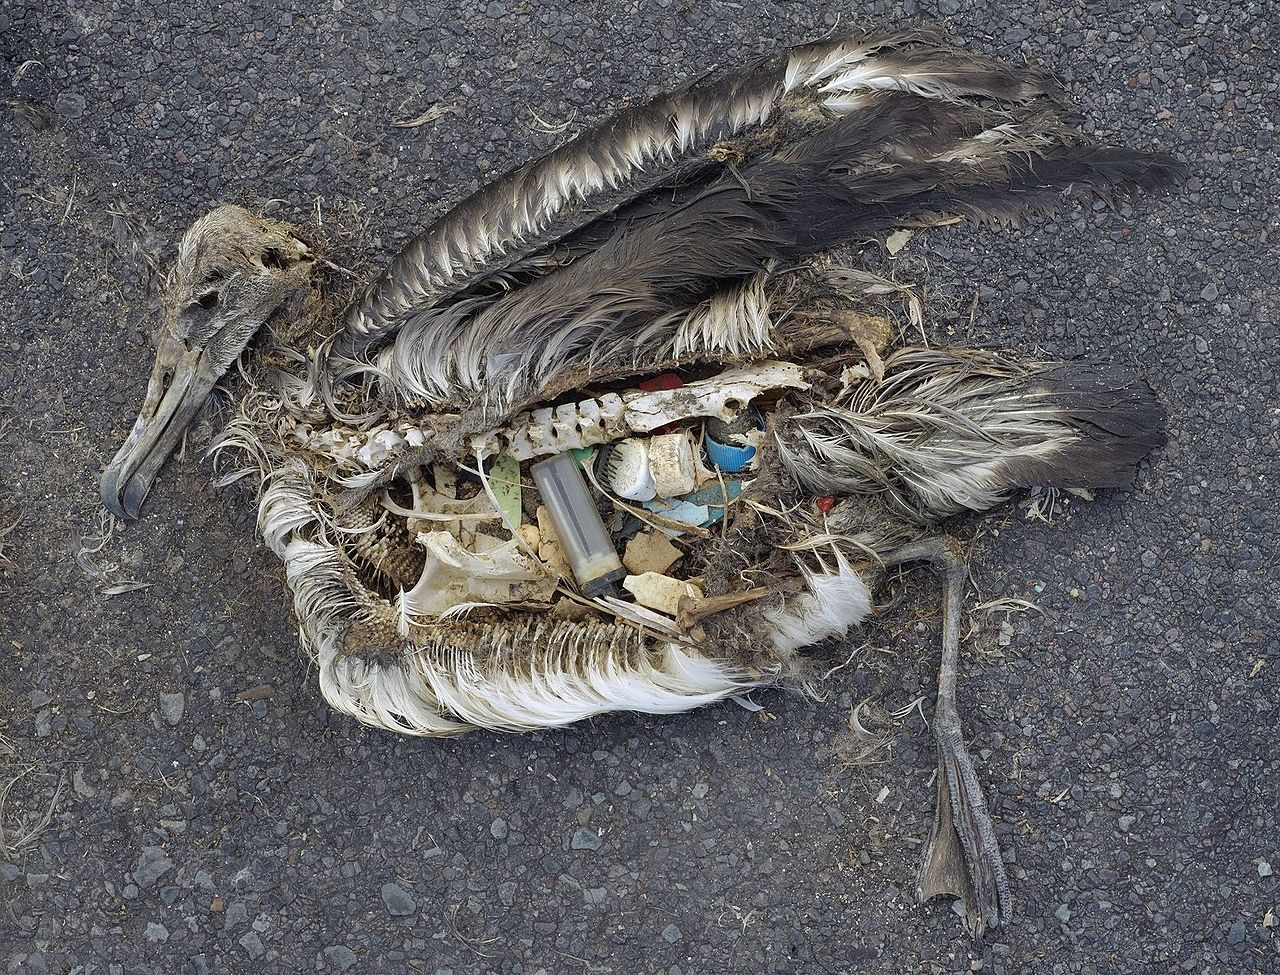
\includegraphics[height=6cm]{graphics/ChrisJordan-Albatross.jpg}
  \caption{Chris Jordan, Albatross at Midway Atoll Refuge, 2009}
  \label{fig:ChrisJordan_Albatross}
\end{figure}

The unaltered stomach contents of a dead albatross chick photographed on Midway Atoll National Wildlife Refuge in the Pacific in September 2009 include plastic marine debris fed the chick by its parents.

Using spare narration and stunning imagery, Chris Jordan's feature film MIDWAY explores the plight of Laysan albatross plagued by the ingestion of our plastic trash. Both elegy and warning, the film explores the interconnectedness of species, with the albatross on Midway as a mirror of our humanity.

Even if garbage leave outs our life, we do not care about the results of it. And it is captured by the works of Chris Jordan.In this photo series it captures 


% Effect of plastic on wildlife in Antartica.
% Her ne kadar biz çöpü attıktan bizim hayatımızdan çıksa da yok olmuyor. Sadece başka bir yerlere gidiyor. Mesela kuşların midelerine. Chris Jordan'ının imageları bunu çok da güzel açığa çıkartıyor. Bizim çöpleriminde habersiz hayvanlar bunları yiyorlar. Bir yandan ürettiğimiz ürünler ile kaynakları tüketirken bir diğer yandan ise artıklarımız diğer yaşanları tüketiyor. Dikkat çekmek istediğim nokta aslında ekolojik hassasiyetlerden çok aslında elimizde avucumuzda ne varsa onları tüketiyor olmamız. Karşı durduğum nokta ise tam olarak burası. 


%****************************************

% First one is actually is to analyze what is trash? Because I am using trash material and what is point of view of scholars to the trash. Realizing the potentials of it. Also the difference comes from the working on virgin object and trash object. Çöp kendi geçmişini falan taşıyor. Yeni blank bir şey değil aslında. Boş bir kağıda resim yapmak ile başka bir kağıdın üzerine resim yapmak arasındaki fark gibi bu. If trash has multiple life than these research will somehow reveal it. It is actually research on trash. I guess it is missing? Yani sanatın dilini genişleten yeni bir soru gündeme atan bir iş değil. I need to set a purpose for the theory chapter. Or it is a just a background chapter?

% Genel anlayışın tersine --- çöpün değersiz, iğrenç, uzak durulması algısına --- karşıt değerli olabileceğini, bir kaynak olduğunu iddia ediyorum, tıpkı bu sanatçıların işleri gibi. Genel göürüşe meydan okuyorum. Sizleri gerçekten bunların değerli bir şeyler olduğuna vs. ikna etmeye çalışacağım

% Ben bu bu bu methodlarla bu işi geliştirdim. Bir dert var o dert üzerine (şu yöntemlerle) sorgulamalar yapıyorum. 

%........................................





%****************************************
% Rubbish: the archaeology of garbage. rathje1992rubbish
% [Refreshed ideas] Garbage project's findings have supplied a fresh perspective on what we know --- and what we think we know --- about certain aspects of our lives. p.24

% The basic methods of garbage disposal are four: dumping it, burning it, turning it into something that can be useful (recycling), and minimizing the volume of material goods. p.33

% ancient peoples p.33

% fast food packaging. p.97

% human behavior p.55 can you tell a lot about the customers from their garbage?

%p.191-192 people tend to think of "recycling" as a relatively modern conceit that has only recently gained broad public acceptance, and whose practical benefits have only just began to be realized. Recycling itself is probably as old as --- indeed, seems to be a fundamental characteristic of --- human species.

%p.209 The reuse of paper, for example, involves processes that generated a considerable amount of hazardous waste. In order to recycle newspapers, magazines, and, indeed, any printed paper, the paper must first be de-inked. At the end of the de-inking process one is left with essentially two products: on the one hand, de-inked fiber that will be turned into new paper; and on th other, a large quantity of toxic sludge.
%........................................


%****************************************
% trasformations 

% during great depression, I learned firsthand about frugality as a child during ww2. my family carefully folded the wrapping paper from gifts to reuse on other occasions. p.8

% p11. for decades we've taken for granted used cars and old houses. Is there anyone alive who has always lived in new houses or driven only new cars?

% p.11 Economics has always been a factor in recycling. 

% p.12 recycling is not limited to folk art. 

% Use of recycled materials is not new, not is it exclusive to the united states. p.18

% p.22 Material, meaning, and memory --- these are artists' reasons for using found objects.

% p.48 recycling may be the most wasteful activity in modern America --- a waste of time and money, a waste of human and anutral resources. john tierney, "What a Waste," seattle postintelligencer...
%........................................





\paraphrase{The names we give this material ---waste, garbage, refuse, trash, rubbish--- have pejorative definitions. Worthless. Rejected and useless matter of any kind. Unimportant. \cite{zimring2012encyclopedia}}



[Trashing Habits] Various objects become trash after their primary functions consumed. People do not care the package of the objects that they buy. They buy the coffee not the cup of it. After coffee finished the life of cup also finishes. They are actually packages that are used to carry or protect other materials. After real material used these packages became valueless (or useless).



[LIFE OF OBJECTS] Objects life time in the nature is more than human being. People use them for just 5 minutes. However, they continue to exist on the nature through the years becauseof they are the result of highly complex industrial production methods and They are not easily decomposable items in the nature. 


% Şu anda lazım değil.
[Biodegradable] \comment{Biodegradable matter is material capable of being decomposed by bacteria or other biological means. Biodegradable  matter usually consists of organic materials such as plant, animal, and other substance matter originating from living  organisms. It has the ability to be broken down into smaller, harmless products by way of the action of living organisms.  The term is often used in relation to ecology, garbology, and waste management. Biodegradable products are often associated with perishables (products, food, and waste materials subject to death or decay). The term biodegradability of a product  refers to its disposition to disintegrate as the result of natural processes.}



% Bu kısma hiç gerek yok.
[Different types of trash] The complexity of produced trashes of societies is increasing. For example developed countries that have nuclear plant generates radioactive wastes which highly hazardous for the environment is never exist previous societies. Think batteries and so on.  It can be thought that when the complexity of trashed increased required effort to repair, reuse and recycle is also increase. Therefore for the ones that have no complex tools it is becoming harder to reuse objects. In other words objects become more complex their re-usage becomes less likely.  Different production process generates different types of trash. According to production process, decomposition process\ldots The approach to the different type of trash will be different. In other word if trash is a result of classification of objects, it can be easily extracted that there is classification inside of it. There are some trashes that are more close to the people. More easy to convert them. more easy to regain to the society. 



%****************************************
% UPCYCLING:
% Burada da upcycling kullanıyor aslında. http://www.gwynethleech.com/cups/suspended
% Raw+Matrial=Art burda da upcycling deniliyor.
%
% RECYCLING:
% recycled, re-seen book.
%........................................




\todo{throwaway spirit (vance packard)}

[Unprofitable, Value, Definition] Waste is considered as something useless, something no longer has value; something sufficiently degraded so that the cost of reclaimation seems higher than the cost of disposal, in other words, something unprofitable. 

[Determination] \paraphrase{The value of things rises and diminishes according to the work they do or the feature imagined for them, in other words, to their potential realized in time. Waste by Willian Viley.}

We are very good at producing waste as well as hiding our garbage. 

[Question] Is it trash or trashed? Is it waste or wasted?

% CHANGE
\paraphrase{In the late twentieth century, in the context of increasing environmental awareness, this consciousness has altered yet again, and waste has ‘been revalued and recoded from rubbish to recyclable resource, it has moved from the bin to the compost heap, it has insinuated itself into our lives in different ways and with different effects’ (Hawkins 2006: 5).}

% Reference from Identity, mobility and the throwaway society
% Resource is here: mmmacleo2005.pdf (throw away culture ile ilgili.) (Çünkü ben bunun ürününü kullanıyorum.)
\paraphrase{In this thesis the undeniable matter of waste, itself pressing, urgent and excessive, is used to infer the presence of a society defined by its generation; a society ceaselessly discarding and abandoning its surplus as excess, as part of an endless desire for the new. Morally corrupt and unequivocally environmentally damaging, the rhetoric of the throwaway society classifies discarding as intrinsically bad and commands us to assume control of our wasting, suggesting the adoption of heightened regulatory practices around disposal as the means to ensure that we clean-up our act. The thesis, however, lacks depth and provenance. It is, actually, glib. Indeed, to infer the presence of a throwaway society from contemporary levels of waste generation is problematic for at least four reasons.}



%****************************************
% MOVE TO CHAPTER 4
% HAKAN GÜRSU, ZIZEK
% Buraya aslında bir de Hakan Gürsu koymak gerekli olabilir. Yani aslında kendisi pek de sanatla ilgili bir laf etmiyor. Ama aslında tükettiğimiz onlarca şeye karşı bir tavır yaklaşım sergiliyor. Bu yüzden theory kısmında yer alabilir. Bu çöpün içinde boğulacağımızdan bahsediyor. Onu dönüştürmek gerekliliğinden yeteneğinden bahsediyor.
%........................................


%****************************************
% TEZ STATEMENT. Dönüştürme
% Ya gerçekten çöpü dönüştürüyorlar ya da çöpe dair düşünceleri dönüştürüyorlar, ve bunu ele alırken aslında heykel, kolaj, fotoğraf gibi şeylerden yararlanıyorlar ama aslında ortaya koydukları şey bir sanatsal eylem. veya bunu sanatsal eylem bağlamında ele alabiliriz.


% Dönüştürme çok temel bir şey ve çöpe çok bağlı. Çünkü değeri sıfıra inmiş bir şeyden bahsediyoruz.
%........................................


as trash live longer than human being, next generations have to cope with previous generations trash. 




[Inspired Works] There are some works that inspire me a lot when developing the work. They are not actually trash related works therefore I put them in different section and here before the details of my work. However the previous chapter has also very inspirational contributions to the my work. They helped the understand the topic and develop an approach to the topic. In this section some projects are mentioned and their methodologies are explained. How are these works effected my work. What is the relationship between them? (Maybe all of them can be explained only the related part of it.)




Recycle the Classics, BY DORIS SOMMER

Trash as History/Memory, Encylopedia, bullock2012trash

John Scanlan's book, On Garbage shows how western progress always has cleared away and discarded what went before; not only material waste but also knowledge. He believes that by examining our garbage we can gain useful insight into the condition of contemporary life.

Book: Recycled, Re-Seen: Folk Art from the Global Scrap Heap






%****************************************
% RESOURCES:
%
% Plagiarism check: http://mashable.com/2012/08/29/plagiarism-online-services/
% What is Plagiarism: http://www.plagiarism.org/plagiarism-101/what-is-plagiarism
%
% How to cite epigraph: http://blog.apastyle.org/apastyle/2013/10/how-to-format-an-epigraph.html
%
% Artist ve artist statementlar için kaynak:
% - http://www.amandadonahue.com/artist-statement/
% - http://www.smfa.edu/cyclo-show
% - http://www.gwynethleech.com/statement
%........................................





%**************************************
% HERE Same sample phrases are listed you can use them:


% The work that follows is divided into three sections


% The artist thinks, acts, performs music, and writes outside the framework that society has created.


% This thesis takes a rather different approach to the resonant possibilities of discarded things. It looks to philosophical ideas and our entangled experiences of things, time and stories, which need to be traversed in order for a discarded object to be called ‘waste’.


% I also want to suggest a different way of considering trash. Maybe art maybe suggest an alternative way of seeing.


% I’d like to criticize a set of concepts or ways of thinking about discarded things that to me just don’t seem quite adequate.


% In an effort to expand art activism's capacity to create real social change, this article will (1) examine the theoretical framework behind art activism and art's efficacy in accessing emotional pathways; (2) explicate ways to strategically approach art activism through the use of specific case studies; and (3) explain one practical form of art activism-theater-based conflict resolution-that is transforming the ways communities are addressing social injustice.


% This thesis is written as a study of the socio-economic change that is currently happening in Serbia, but it’s a study that critically engages with everyday materials that provide the basis for change, rather than the economic development philosophies that are practiced through policy. 


% What specific social issues are you trying to address through Labyrinth?

% The discussions (mentioned discussion are also formed the thesis project entitled ... )


% Aim of this thesis is ...


% There has been a recent spate of artistic work focusing on (over-)consumption using the lens of disposal and discard.


% as a reaction to the consumerist society.


% \ldots is the concern of this study which aims to \ldots


% The aim is not to practice Antiquarian Avant-Garde techniques as a puritan form of photography, but rather to envision new means of photography.


% The aim of the thesis paper is to historically, socially and theoretically contextualize a student's work. The written thesis documents and informs the development and resolution of each student's artistic practice during the MFA program.


% The main aim of the current study was to produce an initial conceptual model that explains 


% The topic of recycling, presented in this issue, is the "re-use" of materials, objects and structures, for different purposes, and in different ways from their original uses, in order to build or re-build, to provide possible solutions to problems related to the environment, and to manage waste more intelligently. Tyres, containers, bottles, cans, CD-ROMs and even keyboards, can find new and unexpected uses in experimental architecture, exhibition pavilions, or low-cost housing. With recycled objects, one can build anti-seismic and energy efficient houses. Recycled materials can contribute towards building shelters to meet the needs of people affected by disasters. There are many topics connected to recycling, and they vary depending on the objects that one wishes to recycle and how they will be put to use. Used tyres find many applications in REfunc architecture and the Bohlin-Cywinski-Jackson studio. Dorte Mandrup transformed a piezometer into the supporting structure for apartments built with standardized modules. David Hertz reused the wings of a 747 as roof for a villa in Malibu. TYIN Tegnestue architects restored a building with recycled materials, mainly found on location. Yatin Pandya and Footprints E.A.R.T.H. built an activity centre in Ahmedabad using items that were considered as rubbish to their original owners. James & Mau and Infiniski designed fashion homes with recycled containers. The same kind of containers were used by MacArthur Studio and Means & Wells, to build a travelling exhibition pavilion. The GAD. In London, Folke Koebberling and Martin Kaltwasser constructed an experimental theatre using only recycled materials. The panorama that emerges shows the extreme heterogeneity of the work, materials and techniques, the intuitive approach and the infinite possibilities offered by recycling. All of these projects highlight the importance of the construction process as an opportunity for learning and discussion. 

% In light of this argument

% To frame a discussion, narrow down the topic

%........................................


My work relation with the other works.

(My work needs to be considered in the context of art. I need to focus on the notebooks establish with art.)

sanki çöplerden bir şeyler yapmak bir şeyleri ispatlamak gibi gözüküyor. Ya da gene bir yetenek gibi gözüküyor. Bulunmaz kumaş misali. Yok abi kimsenin başaramadığı şeyi başarıyorum gibi bir şey yok. Ben ilgilinilmeyenle ilgileniyorum.



\chapter{Uncategorized}


%****************************************
% RESOURCES:
%
% Plagiarism check: http://mashable.com/2012/08/29/plagiarism-online-services/
% What is Plagiarism: http://www.plagiarism.org/plagiarism-101/what-is-plagiarism
%
% How to cite epigraph: http://blog.apastyle.org/apastyle/2013/10/how-to-format-an-epigraph.html
%
% Artist ve artist statementlar için kaynak:
% - http://www.amandadonahue.com/artist-statement/
% - http://www.smfa.edu/cyclo-show
% - http://www.gwynethleech.com/statement
%........................................


%**************************************
% HERE Same sample phrases are listed you can use them:

% The work that follows is divided into three sections

% The artist thinks, acts, performs music, and writes outside the framework that society has created.

% This thesis takes a rather different approach to the resonant possibilities of discarded things. It looks to philosophical ideas and our entangled experiences of things, time and stories, which need to be traversed in order for a discarded object to be called ‘waste’.

% I also want to suggest a different way of considering trash. Maybe art maybe suggest an alternative way of seeing.

% I’d like to criticize a set of concepts or ways of thinking about discarded things that to me just don’t seem quite adequate.

% In an effort to expand art activism's capacity to create real social change, this article will (1) examine the theoretical framework behind art activism and art's efficacy in accessing emotional pathways; (2) explicate ways to strategically approach art activism through the use of specific case studies; and (3) explain one practical form of art activism-theater-based conflict resolution-that is transforming the ways communities are addressing social injustice.

% This thesis is written as a study of the socio-economic change that is currently happening in Serbia, but it’s a study that critically engages with everyday materials that provide the basis for change, rather than the economic development philosophies that are practiced through policy. 
%........................................


%%%
%%%
%%%
\section{In Theory}

% TODO PRAP. REF.
% FROM Recycle the Classics, BY DORIS SOMMER
% Her alanda recycling var olabilir, literatürde de vardır?
\comment{WHAT, WHERE?} Literature is recycled material, a pretext for making more art. I learned this distillation of lots of literary criticism in workshops with children. I also learned that creative and critical thinking are practically the same faculty, since both take a distance from found material and turn it into stuff for interpretation. For a teacher of literature over a long lifetime, these are embarrassingly basic lessons to be learning so late, but I report them here for anyone who wants to save time and stress.

\comment{MOVES} \paraphrase{Igor Kopytoff, a professor of anthropology, introduced the notion of commoditization “as a process of becoming rather than as an all-or-none state of being.” As such, Kopytoff wrote, the biography of an object was considerably similar to that of a person: occupying different positions, leading diverse careers in the course of different periods between a beginning and an end, being defined by different regimes of value that are both economically and culturally inscribed. (Igor Kopytoff, “The Cultural Biography of Things: Commoditization as Process)} \todo{ref.}

\comment{MOVES} \paraphrase{Objects moves around and their values change constantly. (The idea that objects lead social lives was elaborated and discussed in detail in Arjun Appadurai (ed.). The Social Life of Things: Commodities in Cultural Perspective)}\todo{ref.}

% Like a summary sentence
\comment{TRASH MOVES.} Here the important thing is moving nature of trash. Objects moves and gains different meanings through this movement. Sometimes it becomes artwork, sometimes it becomes archaeological part, waits in the dump-site or wait to be recycle. It also signifies that it is relative and result of a classification issue. All of them are creates a harmony. supports each other with different words and conceptualization. 

% <From "Trash Moves On Landfills, Urban Litter and Art" by Maite Zubiaurre
\comment{TRASH MOVES.} \paraphrase{Below part Explains journey of trash, its different steps. Object moves and also trash also moves. How is it life of trash? This part explains life of trash. How does it intersect with other people in which places? This part also can be understand by pointing out different part of it with detailed explanation. For example an artist collect from trash from streets and the other one goes to the (For example Vik Muniz) landfill. In other words there are different places to touch on trash. Every place generates different story? Or to understand it more deeply it covers different part of it. Or provides ideas about it. Lots of people touches it from philosophers to artist. Also in the later parts it draws attention to them.}

% Ama çöp olarak zaten kalmıyor bu trash bir şekilde hayatımıza tekrar giriyor. Ne kadar itise de... Trashion: the return of disposed. trash moves. Peki geri dönüşü nasıl bir değişiklik yaratıyor. Ya da gerçekten geri geliyor mu? Kullandığımız ürünlerin ne kadarı tek kullanımlık. Tek kullanımlıklarla nerede karşılaşıyoruz. Evet belki hayatımızda çok kullanılan şeyler var fakat. daha tek kullanımlıklar da var denilebilir.
\comment{TRASH MOVES.} \paraphrase{Trash moves, all the time. It becomes a steadily growing heap of clutter behind closed walls, accumulates and festers under tight lids, travels from a small trash can in the kitchen to a large one on the curbside, joins other people’s rubbish when the garbage truck arrives, drives to the transfer station, where it circles around on conveyer belts, bids farewell to recyclable or composable goods, is loaded (if declared useless: the ultimate trash) into yet another garbage truck, or barge, or even train, until it arrives at its final destination: a sanitary landfill. Even in the landfill, it does not remain still. Monster "waste handling dozers" move rubbish around, compact it and press it against the soil. More importantly, they incessantly “sculpt” refuse with their huge shovels and caterpillar wheels, making sure the garbage mound does not tip over to create a fetid avalanche. When night falls, and the trash load of the day finally disappears under a thick layer of mud, detritus still moves: once underground, it settles differently, and decomposes at a different speed, thus continuously altering landfill topography: where there was an even plateau, now there is an abruptly descending slope, and a valley; and where there was a perfectly smooth road, now there are deep crevices in the pavement. This is how trash moves. But\ldots who moves on trash? In the United States, it is mostly big-wheeled machines, an industrious army of giant yellow insects busying themselves on a heap of rubbish. In Latin America, it is mostly people. People who hand-pick garbage, who build their shacks on densely compacted trash layers, and who, day in and day out, eagerly throw themselves into the boisterous cascades of fresh debris falling from garbage trucks. In many of the garbage dumps around the world, scavenging becomes a steady job. \quotes{Garbage properly \quotes{stored} and put away brings peace of mind, as do corpses boxed and buried, or criminals confined to a cell.} And thanks to Art: for Art shows how trash--even the one that stops moving, and particularly the one that lies squished, squashed, and weathered, almost fossilized, on the ground---has the potential to move: to move us, that is. (through the works of Filomena Cruz's photographic series “Road Kill”)}
% >

\comment{WASTE AND TECHNOLOGY RELATIONSHIP} \quotes{We live in a badly engineered world, because the vast amounts of waste (both material and energetic) are needless; and that waste could be virtually eliminated through better design} \cite{mcdonough2010cradle}. In other word the problem is our technology which is not perfect. (and I'm not sure that at some point that technology will reach to the perfection or not.)

% WHO OWNS TRASH? kısmı benim işimde sorgulanabilir, ya da ünlülerin trashlerini inceleyen adam kısmında ele alınabilir. Orada aslında başkalarının trashlerinin insanlar hakkında neler anlattığını çok güzel anlıyoruz.
\comment{ANALOGY Between landfill and graveyards. WHOSE TRASH?} \quotes{There’s a relationship between graveyards and landfills, one that makes us uncomfortable, Zubiaurre explained. \quotes{What is happening to trash is what is going to happen to us. We’re all going to end up in a dump, and we’re going to decompose. That’s the ultimate destiny of humankind, and we don’t want to face that.} Trash is also regarded differently, depending on where you live. Last year, an undergrad in Zubiaurre’s honors collegium seminar went to a poor neighborhood and scavenged through people’s trash; no one cared, Zubiaurre said. But when the same student went to Beverly Hills to go through trash, the police were nearly called. \quotes{Who decides what is public and what is private? How come trash becomes highly private in a rich neighborhood, but truly disposable in a poor neighborhood?} Zubiaurre said.} \cite{zubiaurre2015trash}

\comment{TRASH AND OTHER DISCARDED NOTIONS} From my point of view and approach in this thesis, trash is only one of the thing that is being discarded by humans and communities. There are lots of things that are being excluded such as homosexuals, trans, disabled peoples etc. Even if they are excluded, there is also life for them. 

% TODO Reference
\comment{WHAT?} John Scanlan's book, On Garbage shows how western progress always has cleared away and discarded what went before; not only material waste but also knowledge. He believes that by examining our garbage we can gain useful insight into the condition of contemporary life.

% FROM Culture, Values, and Garbage, Encyclopedia 
\comment{INTERACTION WITH GARBAGE. VALUE SYSTEM, DECIDING TO GARBAGE.} \paraphrase{"The Trash Talk project emphasizes the complex, yet overlooked, relationships that garbage and people share. In terms of their relationship to garbage, all people interact with it on two levels. One is a material connection, indicative of the physical and sensory contacts that people have with garbage. In some households, this connection begins with an individual removing an item from packaging, disposing of that item in the kitchen receptacle, placing that item and others into a larger bin, taking that bin to the curbside, and then the material connection ends. Others, including workers in sanitation plants and recycling centers, then continue a material connection with the garbage, but the material connection of the consumer and the garbage ends with the bin on the curbside. The second connection that people maintain with garbage is an ideational one. Unlike the material one, which is manifested in things that can be touched, moved, and sensed, the ideational connection operates on the level of cognition. The differentiation of an item of value from an item of trash, for example, has nothing to do with the material principles of the object. Instead, humans determine whether the object is of value or whether it is considered trash. The decision of whether an individual decides to dispose of a broken radio or to consider it an heirloom to be kept is highly subjective and rooted in the value systems of a culture." "After the item is eaten, the individual has to decide what to do with the remainder, such as the leftover package. The package might be reused, re-purposed, or recycled but, most likely, will be disposed of in the trash." \cite{lukas2012culture}}

% FROM Garbage in Modern Thought, Encyclopedia
\comment{THROW AWAY CULTURE.} \paraphrase{"Philosophers and intellectuals have expressed the need to focus on the centrality of garbage, but for everyday individuals, the understanding of garbage is often as something “out of sight, out of mind.”" "Modern humans, as part of their penchant for consumption and unsustainable living, often think very little about the waste that they produce." "Like many aspects of capitalist living, the person throwing away a piece of trash does not connect the various levels of production, consumption, and post-consumption involved in the trash. It becomes a secondary matter---an afterthought." "Martin O’Brien, among many thinkers, argues that the understanding of garbage should be a central concept, especially since garbage typically correlates with social change, social roles, and institutions. Thus, beyond the level of individuals and their relationship to garbage, there is an interest in understanding the central role that garbage plays in all of society’s roles, institutions, and forms of change." "Garbage is excess--- it is a part of society that society no longer desires." \cite{lukas2012garbage}}

% FROM Garbage in Modern Thought, Encyclopedia
\comment{CATEGORIZATION.} \paraphrase{"Garbage is categorization, according to Susan Strasser." "In recycling programs and in places of refuse disposal, items of trash are categorized depending on their potential value, possible environmental harm, or time of decay. Consumers have become accustomed to the categories that are often applied to garbage. Many cities require people to dispose of their garbage in an orderly fashion---perhaps separating wet household waste from dry---and recycling programs ask individuals to divide their recyclable items into sets (such as plastic, glass, aluminum, and paper) and smaller subsets (such as PET or 01, PE-HD or 02, and PVC or 03). Garbage is an illustration of how humans use mental categories to order the material world." \cite{lukas2012garbage}}

% Garbage is universal, reference
\comment{NO VALUE, UNIVERSAL} \paraphrase{"According to John Scanlon, garbage is indicative of a separation of the world---the desirable from the unwanted. Michael Thompson uses the riddle of the rich and poor person’s approach to snot (one keeps his in a handkerchief, the other disposes of it with a tissue) to underscore the curious ways in which garbage is connected to the issue of value. While garbage is universal---all societies, extinct and extant, have produced or produce garbage--- the conditions under which garbage is understood are culturally determined. Many non-Western societies attach a much greater value to items after they are discarded. In the United States and many other nations, garbage often results not because something no longer has utilitarian value but because the item in question is defined as something of no value. Thus, garbage is not only an objective condition of material culture, but also a subjective one of mentalist culture. People define what is trash and what is valuable." \cite{lukas2012garbage}}

% Hepsinin ayrı bir manası olması falan.
\comment{Semiotic Context, juxtapositions} \paraphrase{"In popular writing (such as novels), in television, films, music, and other forms of mass expression, the term trash is used to signify work that is of especially low value." \cite{lukas2012garbage}}



\comment{read resource (Trash as History/Memory) \cite{bullock2012trash}}

% Walter Benjamin's trash aesthetics and Adornos reflection? Bu konudan ben hiç bir şey anlamadım açıkcası. Çünkü ne dedikleri ne yaptıkları hiç belli değil.
\todo[inline]{BU NE OLACAK? NEREYE BAGLANACAK, GARBOLOGY??}\paraphrase{\quotes{Benjamin’s approach to history is through \singlequotes{trash}---through the spent and discarded materials that crowd the everyday}  \cite{highmore2002thrashaesthetics}. Benjamin’s importance as a theorist of the everyday is most evident in his attention to the everyday experiences of modernity. In the face of the endless proliferation of trash, Benjamin potentially suggests a \singlequotes{trash aesthetics} that could be used radically and critically to attend to the everyday. The method might be thought of in terms of \singlequotes{recycling} --- an ecology of everyday experience.}

% FROM Trashion: The Return of the Disposed by Bahar Emgin
\comment{LIFE AN OBJECT} \paraphrase{In light of this argument, one could claim that the end of the life of an object corresponds to the moment in which it is disposed of. This disposal might take place in different forms and for different reasons; however, in the most literal and common sense, the life of an object ends in a trash can in the form of waste. In this moment, the object is left valueless in all the possible meanings of the term value: It can no more serve a function, it can on no account be exchanged for anything else, and it can by no means engage in the processes of signification to connote and endow its user with specific social values.} \todo[inline]{reference, (Trashion: The Return of the Disposed by Bahar Emgin)}

% FROM Trashion: The Return of the Disposed by Bahar Emgin
\comment{REFLOW IN THE MARKET} \paraphrase{Referring to the work of Susan Strasser, Hawkins argues that disposal was central to the logic of mass production and hence should not be assessed as only particular to consumerism in the twentieth century: “Mass production of objects and their consumption depends on widespread acceptance of, even pleasure in, exchangeability; replacing the old, the broken, the out of fashion with the new. The capacity for serial replacement is also the capacity to throw away without concern.”} \todo[inline]{reference, (Trashion: The Return of the Disposed by Bahar Emgin)}

\comment{TECHNICAL PROBLEM, NEED TO MANAGED, RECYCLING (CAPITALISM), UPCYCLING} \paraphrase{On the contrary, with respect to the issue of disposability, waste was handled merely “as a technical problem, something to be administered by the most efficient and rational technologies of removal.” Only through the rise of environmental movements in the 1960s did the disposal of waste come to be loaded with negative meanings and iewed through a moral framework. The enormous quantities of waste accumulating in urban centers, Hawkins writes in “Plastic Bags,” were not only taken as a threat to the environment, but also as a sign of an individualistic, insensitive, and hedonistic consumer society. Waste now became evil. If the environment is to be saved from our destructive power, then waste should be “managed,” Hawkins asserts. Consequently, recycling gained its contemporary prominence “as virtue-added disposal\ldots disposal in which the self is morally purified, disposal as an act of redemption.” Disposal in the form of recycling is now a moralistic attitude through which we pay the debt we owe to the world. Upcycling... On the other side of the coin is the business stemming from these practices; recyclers not only ease their conscience through recycling; they also make a profit. Recycling, as “the huge tertiary sector devoted to getting rid of things, is central to the maintenance of capitalism; it doesn’t just allow economies to function by removing excess and waste—it is an economy, realizing commercial value in what’s discarded,” Hawkins and Muecke write in Culture and Waste. In the same manner, upcycling has already been turned into a business: Certain designers labeled eco-friendly are earning money through upcycling, competitions are organized around trashion, numerous websites are devoted to promoting and selling upcycled objects, and online and print resources explain how to upcycle at home. In short, there is a whole sector of upcycling now.} \todo[inline]{reference, (Trashion: The Return of the Disposed by Bahar Emgin)}

\comment{DESIGN, ALTERNATIVE DICIPLINE.} \paraphrase{Design, as a conduit of disposal, reintroduces rubbish as objects of distinction, invaluable and potentially priceless. People are often eager to see objects that were once considered useless and tasteless when they have been invigorated with new life.} \todo[inline]{reference, (Trashion: The Return of the Disposed by Bahar Emgin)}

\comment{UPCYCLING, sample thesis statement sentence} \paraphrase{This article is about those objects that are recreated from trash through the process of upcycling. Upcycling is a term used by architect and designer William McDonaugh and chemist Michael Braungart and refers to “the process of converting an industrial nutrient (material) into something of similar or greater value, in its second life.” I argue that design, in this instance, acts as a tool of transformation and reintroduces into certain orders what was once deemed waste. This theory counters the argument that an object is dead once it is disposed of.} \todo[inline]{Reference, (Trashion: The Return of the Disposed by Bahar Emgin).}

\comment{CATEGORIZATION OF WASTE} \paraphrase{Douglas argues that our classification of dirt lies not with what objects are but where those objects are. (Think that the transformation process. Previous argument support that the transformation of trash is possible by changing the place of them. In other words removing them from landfill and waste bins to the book selves accomplish to transform trash.) ‘Dirt’, writes Douglas, ‘is the by-product of a systematic ordering and classification of matter, in so far as ordering involves rejecting inappropriate elements’. For Douglas dirt is a spatial problem, a question of not what stuff is but where it is.} \todo{Reference, (Waste by William Viney).} 

\comment{CATEGORIZATION OF WASTE} \paraphrase{“Dirt”, writes Douglas, “is the by-product of a systematic ordering and classification of matter, in so far as ordering involves rejecting inappropriate elements.” Dirt is only dirty in certain places, when it is out of its correct position. Just as faces, for example, is considered dirty when it is in our kitchens but not when it is in our bodies, so it is that our classification of waste depends on the location of objects.}  \todo{Reference, (Waste by William Viney).}

\comment{CATEGORIZATION OF WASTE} \comment{susan strasser ile douglasın fikirlerinde bir ortak nokta görülebilmekte. Özellikle trashın relative olması ve bu işin aslında bir ordering and classification olduğu konusunda. Remember the example given: shoes  on the dinner table.}

\comment{CATEGORIZATION OF WASTE} \paraphrase{waste is “matter is out place”, a definition first given by Lord Palmerston in the mid-nineteenth century and incubated by the British anthropologist Mary Douglas, in her book Purity and Danger.}

% https://narratingwaste.wordpress.com/tag/king-lear/
% Not all waste is dirty, it not always dangerous, contagious or abject. \ldots waste might be quite useful in making time and in keeping time.

% Cornelia Parker's work, narrate an absent event of waste
% There is also strong relationship with the collecting discarded stuff and archeologies of waste.

%%%
%%%
%%%
\section{In Art}

\comment{Crowdsourcing artworkümde neden insanlardan topladığımı, neden onları kullanıdığımı anlatacağım yer ile ilgili olabilir.}

%*************************************
% Phrases...
% What specific social issues are you trying to address through Labyrinth?
% In view of the diversity of online crowdsourced art projects, as illustrated by the examples cited so far, it is useful to map out this artistic trend by developing a comprehensive and multidimensional typology of online crowdsourced art. Table 1 organizes this classification according to a set of multiple criteria. (But this one can be used at introduction, but it is too long to fit on introduction. Maybe select works by giving prominence to some of the features. So the approach to the trash is going to be introduced and also it is reveals the what i am doing in this context.) (A Typology of Online Crowdsourced Art. Diye bir örnek var aslında benzer bir şekilde bu trash içinde yapılabilir.) 
\subsection{Crowdsourcing, Participation, Open Work}
\todo[inline]{TODO needs reference, FROM Crowdsourced Art and Collective Creativity}
In the words of Jeff Howe (2006b), the Wired columnist who coined this term in June 2006, \quotes{crowdsourcing represents the act of a company or institution taking a function once performed by employees and outsourcing it to an undefined (and generally large) network of people in the form of an open call}. The vital elements that qualify an outreach strategy as crowdsourcing are, according to Howe, the use of the open call format and the reliance on a large network of potential workers. Although in some cases there is a material reward for the best contributions, the existence of financial incentives is not a required feature in crowdsourcing. Because of the diversity of its applications, crowdsourcing continues to be a disputed term in both the scholarly literature and the popular press; Howe’s original definition is, in this sense, a helpful delineation of its practical sphere.

The value of crowdsourcing lies in the collective intelligence of the contributors. Pierre Levy (1997) describes this concept as “a form of universally distributed intelligence, constantly enhanced, coordinated in real time, and resulting in the effective mobilization of skills” (p. 13). The question of collective intelligence—and its potential efficiency in various practical settings—has received much attention in both academia and journalism. Researchers studying team performance generally agree that, under the right circumstances and with appropriate motivation, large groups of people can work together and harness their collective intelligence to achieve efficient results (Benkler, 2006; Rheingold, 2002; Surowiecki, 2004). Nevertheless, artistic creativity is different from innovation and intelligence, and it requires a unique set of skills and sensibilities as well as a particular type of cultural capital; if we admit that crowds can have collective intelligence, do they also have collective creativity in an artistic sense?

All these pages are rescued and with their [hi]story they are separated from unused new produced blank sheets and notebooks. They are not bought, not gift. They are found. They are accepted. One of the most creative medium is paper and pencil. Chance given to the people through this work.

However, in view of its reliance on the artistic contribution of a large pool of usually anonymous participants, this type of art raises important questions about notions of collective creativity, authorship, collaboration, and the shifting structure of artistic production in the new digital environment. It is well studied area. Pick a method here. Transforming trash with collaboration.

As curator Andrea Grover notes, “having the audience become co-creators is not a new impulse”; the Internet simply offered a new platform to accomplish this goal (Strickland, 2011, para. 5).

Here this question can be raised about why this type collaboration. Another option can be working together with people on a table. Creating things at that time and transforming the objects here. Possibly the connection to the people will more realistic and intense. However same things can be succeed on the internet at some level. 

While crowdsourced art challenges the traditional role of the artist, it simultaneously redefines the conventional function of the public, turning them from passive receivers into engaged producers. (This totally a new area to discuss, I'm going to summarize and introduce concepts and debates. How are they support my work and how they are give way to me?)

% This article therefore aims to fill these critical gaps by analyzing the practice of online crowdsourced art within a framework of collective creativity and participation theories. Principally, my interest is in answering two key questions. What is crowdsourced art and how can it be classified? And how does the structure of the artwork determine the degree or significance of participation?

% why collaboration, is it really a collaboration? It is methodology used in my practice. 

% TODO: Umberto Eco's Open Work


%*************************************
% ARTWORKS:



% Dark Matter: Explosive View.

%.....................................


%*************************************
% Solid claims about its cultural aspect.
\subsection{Book: Recycled, Re-Seen: Folk Art from the Global Scrap Heap}
\comment{GIFT FROM GOD, NOT KNOWING PREVIOUS STATE} They also states that the practice of tribal people artfully transform Coca-Cola bottle (given as example by the authors). From western trash to tribal treasure. \paraphrase{For the Kalahari Bushmen, the process appears to be one not so much of reusing but of creating anew; not so much transforming, a inventing (p.9).} It stated these found objects is accepted as a gift from gods. A disposable item becomes imminent desire and profound social consequence. (Intercultural recycling.) \paraphrase{Both presentations tell a story about an aesthetic and cross-cultural process --- as well as an economic and political one --- which is defined by the act of recovering and transforming the detritus of the industrial age into handmade objects of renewed meaning, utility, devotion, and sometimes arresting beauty (p.10).} 

\comment{HYBRIDITY} They claim that \paraphrase{the end result is a category of hybrid objects that bear the mark of at least two distinct domains, each with its won material, meaning, makers, and users (p.10).} (some of them utilitarian, some of them ornamental.) \paraphrase{Whatever their ultimate function, each of these objects contains within itself a visual, material, and conceptual reference to multiple technologies, histories and temporalities.}

\comment{SEMIOTIC CONTEXT} \quotes{Like collage in art or quotation in literature, the recycled object carries a kind of "memory" of its prior existence. Recycling always implies a stance toward time --- between the past and the present --- and often a perspective on cultures --- one's own and others. (Jacknis 1992)} \todo{ref.}

\comment{HYBRIDITY} \paraphrase{It is stated that same object can have one meaning for one community or culture and another meaning or series of meaning for another. Different objects have different life spans --- different degrees of permanence or disposability --- and that these life spans are socially constituted is also an integrated part of the story \ldots geographic and socioeconomic boundaries of class, caste and culture throughout the world. It is story of people --- the women, men, children etc. one person's trash into another's treasure.}

\comment{OTHER DICIPLINE, INDUSTRY} \paraphrase{the process of re fabrication explored here is not to be confused with the kind of industrial strength recycling to which we in the West are most accustomed. When we think of recycling in America and other industrialized nations we imagine an automated sequence beginning with the curbside disposal of aluminum cans, plastic bottles, and old newspapers. returned to the industrial process. solid waste management, global greening, and ecological awareness are the buzzwords that guide and motivate consumers and industries to engage in this process of secondary and post consumer waste recycling.}

\comment{DIFFERENT SCALES OF RECYCLING} There are different kinds of recycling that is small-scale, hand done, and local --- a kind of recycling in which yesterday's newspapers are transformed by hand into tin trunk liners;empty food cans become kerosene lanterns; and old tires are refashioned ... 

[Having different meanings] For the same people are not used the items that are scavenged by people who have little or no contact with those who first possessed them, and may neither know nor care about their originally intended function. It is case from the film and also the case depicted in the real life photographs taken by anthropologist michael leahy which document his first colonial contact with new guinean highlanders 

\todo[inline]{yerlinin fotoğrafı}
\quotes{Renowned early-twentieth century anthropologist Michael Leahy encountered a Wabag man from Papua New Guinea wearing an aluminum whole wheat biscuit tin on his head. In the symbol system of this culture, large, bright, and shiny ornaments are connote health, well-being, sexual attractiveness, and the approval of the ancestors.} \todo{ref.}

\comment{CONSUMER CULTURE} \paraphrase{We are dealing specifically with industrially produced consumer discards and their subsequent transformation, these essays are necessarily situated in a particular time, place, and sensibility: the consumer culture of the late twentieth century. In its most basic form, I refer to a consumer culture as one "in which the activities and ethics of a society are determined by patterns of consumption" rather than production (Mamiya 1992, 2)}

\comment{CONSUMER CULTURE, SORUCE OF TRASH} While consumption has provided a foundation for the transnational capitalist system adntheus has much longer history than the last fifty years this thesis focused on the more recent history. because it is during the history of consumption. consumption can be though that as global not to a western or first world countries.

\comment{GLOBAL} It is not limited with geography, ethnicity, gender, nationality. The process of of retrieving and transforming a consumer package or product that someone else has thrown away is a phenomenon that is taking place in the largest metropolises of urban America as well as the remotest corners of amazonian rain forest. 

\comment{GLOBAL, SELECTING COMMODOTIES, } To frame a discussion that incorporates an understanding of such diverse locations, objects, and peoples is to claim links between material process that originate under vastly different social, economic, environmental, and political circumstances. \ldots The most obvious link are the raw materials the raw materials themselves: the packaging, broken pieces. becomes raw materials for other things. these consumer items. and it is spreated globally. It can be seen remotest corner of the world. the indigenization of western objects. (sahlins, 16) Do these hybrid objects, as many western critics might assume, point to passive acceptance of a homogenized consumer culture in the service of western capitalist expansion, or, even worse, a sense of want and deprivation when confronted with "our riches"? Marshall Sahlins: "The first commercial impulse of the local people is not to become just like us, but more like themselves. They do not necessarily despise our commodities. But they are selective in their demands and transformative of their uses of such things. (sahlins, 13)" 

\comment{People applies their own perception to interpreted the items.} Human manufactured never envisioned possibilities seen by people. It suggests a self-confididence and intellectual authority that allows local peoples to encompass western goods in their own meanings "in their own scheme of things." 

\comment{IRONIC, maybe added to results of transformation, reusing trashed items in different contexts.} This misuse the detritus of the industrial age has been described by western theorist as ironic. the irony is often embodied visually and conceptually. opposite of natural use, expected perception. for example making something from nothing or turning trash into treasure. By juxtaposing different materials changing context and place. 

\quotes{It is clear that one man's rubbish can be another man's desirable object; that rubbish, like beauty, is in the eye of the beholder. (thompson, 1979, 97)}

[initial function throw away society] \comment{Karşı çıktığım şeylerden birisi objelerin ilk manaları, ilk kullanım alanları. many scholar stated the general attitude in the society. It is key ingredients of throw away society. initial function is fulfilled by }

\comment{How does it become trash?, initial function.} when an object is discarded it is perceived as being no longer of value to the person or society that once possessed it. Once a newspaper is read, or a bottle of soca pop consumed, its initial function is fulfilled and it is intended to be thrown out as trash.

[Chapter 2] rubbish Theory \comment{DEFINITION} Rubbish is, by definition, an object that is not or is no longer, owned by anyone, that falls outside all categories of economics, culture, and social control. As one of many things on the garbage heap, a discarded object even tends to take on a negative value as something unsanitary, dangerous. The socially constructed value of the object has shifted over time from its finite life span of usefulness and meaning to a timeless and valueless of socially sanctioned rubbish. 

[Chapter 2] \comment{Capitalism, market.} The remarkable thing about many of these objects - especially those produced in the last of the twentieth century - is that they were specifically designed to end up on the garbage heap. They were designed to decrease in value over time - to be used one, or twice and than to be thrown away. This applies not only applies packing - designed containers that protect and promote products - but to an ever expanding list of products. themselves. \todo[inline]{Waste and wantta bununla ilgili bir bölüm olmalı.}

[building new things from ruin] \comment{small amount of it} while most waste ends up in these unsanitary and unsightly landfills, some small percentage is reincorparated --- or recycled --- back into the economic and cultural system of the local population. Indeed, this is the power of rubbish as a category of possessable objects: it has within itself the potential of being discovered, retrieved, and transformed back into an object of greater or lesser durability. 

[Resistance] \comment{Resistance, tactile, agnes varda?} If it is ultimately romantic to speak of these toys (or any other modern-day recyclia) in the language of resistance (by which I mean self-conscious political opposition), I would agree with Marshal Sahlins's assertion that "whether or not it comes to this [resistance], the indigenous mode of response to imperialism is always culturally subversive, insofar as the people must need to interpret the experience and they can do so only according to their own principles of existence. (sahlins 1992, 16)"

\comment{hybrid} each recycled object contains within it a reference to two or more distinct times. \comment{not every time actually, if you transfor ok. it applicable for my case.} Whatever their ultimate design or destination, these recycled artifacts are, by definition, "impure", "inauthentic" products of past and present, here and there, "us" and "them" (clifford 1992) \todo{ref.}

[Reasons of recycling] \comment{Economic conditions forces to people recycle and reuse. but even if they have no economical struggle, they continue recycle. what is the reason of it.} Recycling as an economic strategy of survival in developing countries throughout the world. creative production that is motivated, primarily, by adverse conditions of economic necessity. (lanfill orchestra here. bookcovers here.) Economic survival and adaptation are influential factors for both the makers, who build informal business on the making and selling of recycled goods, and the local consumers, for whom the market for affordable, utilitarian goods is devised. (p25)

